\documentclass[12pt,onecolumn]{IEEEtran}

\usepackage{rotating}
\usepackage{tikz}
\usepackage{booktabs}
\usepackage{multicol}
\usepackage{tabularx}
%\usepackage{color}
\usepackage{xcolor}
\usepackage{lastpage}
\usepackage{fancyhdr}
\usepackage{grffile} 
\usepackage{graphicx}
\graphicspath{ {images/} }
\usetikzlibrary{arrows, positioning}
\usepackage{amsmath}
\usepackage{newfloat}
\usepackage{caption}
\usepackage{mathtools,cuted}
\usepackage{lipsum}
\usepackage[final]{pdfpages}
\usepackage{lettrine}
\usepackage{siunitx}
\usepackage{pgfplots}
\usepackage[europeanresistors]{circuitikz}
\usepackage{listings}
\usepackage{verbatim}
\usepackage{pgfgantt}
\usetikzlibrary{arrows}

\lstset{frame=tb,
language=matlab, 
breaklines=true, 
showstringspaces=false, 
columns=flexible, 
numbers=none,
commentstyle=\color{green},
tabsize=3
}

\pgfplotsset{compat=1.14}

\begin{document}
\author{Marion Heimann - 788579 \\ Tristan Kuisis - 812587 \\ Supervisor: Prof Ken Nixon}
\title{ELEN4002 - Lab Project Plan \\ Preliminary Report on the Design and Creation of a Wits Analytics and Visualization of Energy Systems}
\maketitle
\begin{abstract}
    The main purpose of this document is to outline a project plan for the data analytics and visualization of energy systems across the multiple Wits campuses. The multiple energy meters installed across the properties have been gathering data for a number of years. A web server is constructed that is capable of autonomously and repeadly drawing the data from the database. The server will then host a portal that is capable of displaying the data to a user. The web portal will also be used to generate unique visualizations of the data from the sensors.
\end{abstract}
\begin{IEEEkeywords} 
Selenium, 
\end{IEEEkeywords}
\pagestyle{plain}



\section{Introduction} \label{sec:Introduction}
\IEEEPARstart{T}{his} report details the project plan for the data analytics and visualization of energy systems that make up the Wits campuses. 

There are a number of large energy requirements that Wits has-electricity, water, natural gas, petrol, diesel, as well as a number of other resources which make up smaller fractions of the universities energy usage.

This project, firstly makes use of the electricity meters installed throughout the buildings on the properties. These meters have been providing data for varying amounts of time, as well as data outages occurring occasionally (this will have to be dealt with). 
The wealth of information that these data loggers provide allow for the creation of a web server which is capable of drawing this data from the database, and making use of this data to visualize the energy usage across Wits. The web server will be instrumental in allowing a user to visualize this energy in a multitude of ways. 
The timelines, methods, tools, and a number of other details are discussed throughout this report.


\section{Project Specifications}

\subsection{The Data} \label{sec:TheData}
As discussed above, there are a number of energy meters placed throughout the Wits properties. There are approximately 310 data loggers that are connected to the current web portal used by the university. 
The system in place, run by IST \cite{IST}, is based off-campus. This means that their web service and data is housed on their side. All of the data retrieval (from the data loggers) is done through the Wits network and through in some cases through mobile data. This element of the project is discussed further down in sections \ref{sec:DataConversion}, \ref{sec:DataGathering}, \ref{sec:DataManipulation}. 

There are two other highly relevant data sets that will be used for the core part of the project. These are: the energy generated by the solar panels placed on top of a number of buildings throughout campus, and the weather of Wits. 
These two data sets will allow for a unique picture to be painted which further enhances the visualization of the system as a whole. 

Currently, this is the chosen data sets that will be used for the core of the project, however, if time permits, the university holds a wealth of information regarding the location of individuals throughout the university, this is provided with the use of the Integrated Campus Management (ICAM) system which is used for the access control for the university. 
This system is likely to unlock further insights on the universities energy usage and how the movement of individuals affects the energy usage of specific areas. 


\subsection{Back-End} \label{sec:BackEnd}
In order to run the system proposed, a number of operations are required to take place in a selection of programming languages, and all of these should be able to communicate with one another such that the process described by .... can take place. 

The back-end can be described by a local web server that is run on the users machine (in this case, the server is run on each ISTPassword' personal computer), and it is important as it allows the simulation of a server that will (ideally) eventually be placed onto a standalone system such that users with access to the internet will be able to use the system anywhere.
This section is discussed in further detail in section \ref{sec:Server}.

\subsection{Front-End} \label{sec:FrontEnd}
In order to allow for the visualization of energy, the use of standard front-end web tools will be employed in order to provide the user with interaction. 
The back-end will provide all of the processing requirements, and will manage the data. the front-end communicates with the back-end (server) in order to illustrate the required information.
The three main tools (commonly used in any website), are: Hypertext Markup Language (HTML), Cascading Style Sheets (CSS), and JavaScript. 
These three tools communicate with each other and the server in order to provide the user with the required information when viewed from a web browser. 

It is this part of the system where a multitude of visualization tools are used to gain insights into the data. These tools will be discussed in section \ref{sec:ApplicationsAndTools}

This completes the overall description of how the system is constructed and how it functions in order to get the required functionality.


\section{Scope Statement} \label{sec:ScopeStatement}
There are four sections to the scope for this project, these are: data gathering, back-end system, front-end system, and the ability to use the front-end system to gain insights. All of these sections for part of the scope for the project. 

The data gathering system is required to be capable of autonomously and periodically drawing data from the IST server for all of the data loggers and all of the data that they have attained since installation. There are a few details for this section which is left for section \ref{sec:DataGathering} as the system does not always need to gather in the same way.

The back-end system takes part in the data gathering process, this is why it is important that if functions as required. The back-end deals with all of the data storage, as well as processing of the data in order to send it through to the front-end such that a user can interact with the system. This is used as the system which manages the storage and manipulation of the data which is highly important. 
In order to reduce the work required by the client (front-end), the majority of the presentation work will be done on the server, then once it is ready, sent through to the client. 
There may be cases where client side processing will be used, this will be in cases where the visualization tools require it, an example of this will be dygraphs which required the clients browser to interact.

The front-end is important for any web application, as this is the interface which allows user interaction, which is where the focus and importance rests. The front-end makes use of HTML, CSS, and JavaScript to generate the standard format of the system. This configuration is then used with a number of other tools in order to have multiple types of data visualization.
The details of the front-end is discussed in section \ref{sec:WebsiteArchitecture}.

Finally, the fourth key part of the scope is that of the data visualization. This will be done with the use of many tools and methods such that insights can be gained from the data. The most important decision for this part of the scope is that the system should be designed such that a greater understanding of the system can be gained. Two examples of this are: verify that the billing from City power matches that which the system measures, and another interesting, possibly engineering test, is to verify how much energy has been saved with the exchange of the old lights to all LED lights throughout campus. 

% Pick a focus: something to attain (see how money works or how new lights changed things)

Demonstrate concept


\section{Timeline} \label{sec:Timeline}
It is important to illustrate a basic timeline for any project. In this case, the timeline forms a similar order to how the scope is laid out. 
The following list illustrates the important dates for the project, this indicates when certain parts of the project need to be completed. 

\begin{itemize}
    \item 16 July - Project Plan Due
    \item 16 July - Lab Project Officially Begins
    \item 17 August - Deadline to change project name
    \item 27 August - Staff Inspection Day
    \item 28 August - Open Day
    \item 3 September - Project electronic submission deadline
    \item 13 September - Laboratory project conference - presentations and interviews
\end{itemize}

This indicates that there are approximately six weeks in which the project takes place. 
There is a specific method in which the project will take, and this is such that minimal functionality can be gained from the system from the earliest point possible. 
This means that each of the four major sections laid out in the scope will be put together such that the system can be up and running to test out simple functionality. 
This method can be compared to that described in The Pragmatic Programmer, where they illustrate the method of using tracer rounds \cite{pragmatic}, where the use of a full paper design will lead to a successful product, however, in some cases, it may be more beneficial to make use of \textit{tracer rounds} in order to get feedback within a shorter time period and to see the effects of the system quickly.
The nature of this project is such that the requirements from the \textit{client} can be relatively vague, and this type of project is unique as it is quite in it's dataset and use case. 
This implies that many of the tools and methods that are used throughout the project will change over time as there are many unknowns throughout the process. 

These unknowns can be reduced with the use of prior research and comparing similar systems, however, there will always be a non-zero amount of uncertainty for parts of the project.

This is why a lot of prior research and testing has taken place before the project begins. 

The following figure, Fig.~\ref{fig:gantt} illustrates a first estimate on how the project timeline will be structured. The gantt chart is set out in week days, as there are six weeks.  

\begin{center}
    \begin{figure}[htb]
        \centering
        \begin{ganttchart}[hgrid, vgrid, inline]{1}{30}
            \gantttitle{Lab Project}{30} \\
            \gantttitlelist{1,...,30}{1} \\
            \ganttbar{A}{1}{3} \\
            \ganttbar{B}{4}{6} \\
            \ganttbar{C}{7}{10} \\
            \ganttbar{D}{11}{12} \\
            \ganttbar{E}{13}{16} \\
            \ganttbar{F}{17}{19} \\
            \ganttbar{G}{20}{20} \\
            \ganttbar{H}{21}{30} \\    
            \ganttbar{I}{1}{30} \\
            \ganttbar{J}{1}{30}    
            \ganttlink{elem0}{elem1} 
            \ganttlink{elem1}{elem2}
            \ganttlink{elem2}{elem3}
            \ganttlink{elem3}{elem4}
            \ganttlink{elem4}{elem5}
            \ganttlink{elem5}{elem6}
            \ganttlink{elem6}{elem7}
        \end{ganttchart}
        \caption{Estimate Gantt Chart of Project}
        \label{fig:gantt}
    \end{figure}
\end{center}    
Where: 
\begin{itemize}
    \item A - Data Retrieval
    \item B - Data Storage and Manipulation
    \item C - Back-End Setup
    \item D - Back-End Link with Data Retrieval System
    \item E - Front-End Design
    \item F - Integration with visualization tools
    \item G - Reassess System
    \item H - Iterative Methodology
    \item I - Documentation
    \item J - System Testing
\end{itemize}

As it commonly works with gantt charts, there will be tasks which take less time than is scheduled, and they can also run over time, this shifts sections of the chart and effects tasks further down the line.
There are a number of tasks which run throughout the entire project, these are documentation and system testing, this is done as it helps with the development process to run smoothly and any changes that happen to the system are always tested so that different components in the system are not affected with changes to any other system. This testing helps the interfacing of the dfferent components run smoothly, this is discussed in section~\ref{sec:DependenciesInterfaces}.

Finally, there is a task called \textit{Iterative Methodology}, this is where the \textit{tracer bullets} system comes into play, all of the tasks before this are set out to get the system up and running so that vulnerabilities and loopholes can be found in the system, and further visualizations can be added to the system. Once the data sets and the system as a whole is set up, it becomes a matter of working with the data to provide multiple visualizations with that data.

\subsection{Working Times} \label{sec:WorkingTimes}
It has been recommended that the working times for this project should be kept to a standard 08:00 to 17:00 working time, this is done this way so that the project can simulate a \textit{real} project. 
There may be cases where these times will have to be altered such that certain tasks can be completed within scheduled times.

Throughout the project, meetings with the project supervisor, as well as other individuals will take place, these will be used for consulting purposes and follow up meetings with progress on the project.


\subsection{Milestones and Deliverables} \label{sec:MilestonesAndDeliverables}
There are a number of milestones that are used for the duration of the project, these are mostly made up of the major sections in the scope, and are illustrated in the list below:

\begin{itemize}
    \item Retrieval and Storage of Entire Database
    \item Periodic Retrival and Storage of Database
    \item Back-End Setup
    \item Front-End Skeletal Design
    \item Visualizations
    \item Refinement of each stage
\end{itemize}

These are set as the major milestones and deliverables that are currently set out for the project. The nature of the data that is presented by this system affords a highly important resource for major stakeholders in the Wits community. This is why a number of stakeholders have been contacted and asked for their input on the system. 
The input from these stakeholders can guide the later stages of the project as it will be their ideas which determine which are the major visualizations and information that should be inferable from the data.
% Meetings with stakeholders + implement their suggestions


\section{Risks} \label{sec:Risks}

\section{System Architecture} \label{sec:SystemArchitecture}

\subsection{Website/Portal Architecture} \label{sec:WebsiteArchitecture}

\begin{enumerate}
\item Prepare for the activity of sitemapping
\item Brainstorm the types of content
\item Define primary navigation
\item Flesh out second and third level structure and content
\item Don’t forget about utility pages
\item Create notes and high-level specifications for each page
\item Designate the type of design template
\item Iterate. Iterate. Iterate.
\end{enumerate}

Maps which illustrate how one navigates through the website. 

\section{Resources} \label{sec:Resources}

\section{Applications and Tools} \label{sec:ApplicationsAndTools}

\section{Development Approach} \label{sec:Development Approach}

agile, waterfall, scrum

Testing methods


\section{Dependencies and Interfaces} \label{sec:DependenciesInterfaces}


\section{Licensing} \label{sec:Licensing}

\section{Documentation} \label{sec:Documentation}
documentation - each and every part of the system makes use of markdown files which enable users to interact with the system and test it out on their machines. 

\section{Server} \label{sec:Server}
\section{Data Gathering} \label{sec:DataGathering}
weather data

The system has a collection schedule set at thirty minutes, this means that each of the data loggers is sent a request, and the data is the sent to the IST servers, where it is stored in their database. 


IST host a web service which allows customers to view the relevant information from these data loggers. 
The web portal allows the user to view a range of details about the system, the homepage of the system is illustrated in Fig.~\ref{fig:ecwin}.

\begin{center}
    \begin{figure}[htb]
        \centering
        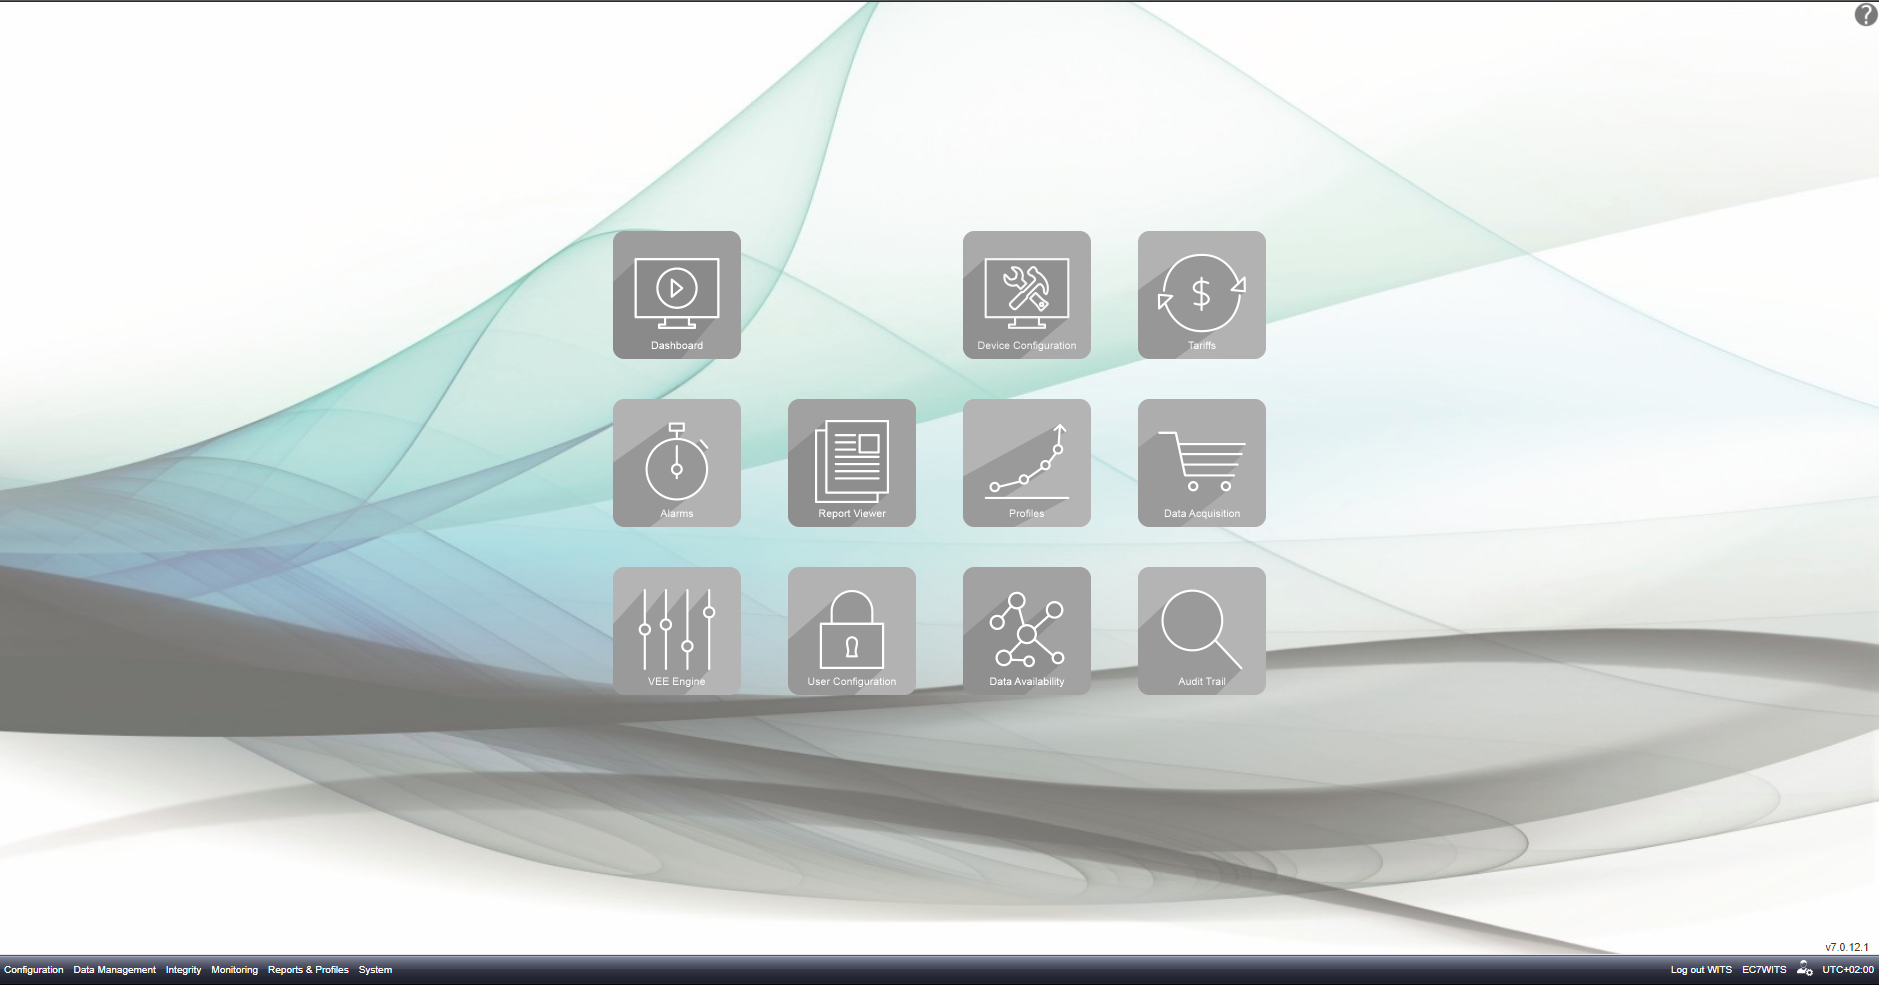
\includegraphics[width=0.8\textwidth]{ecwin.png}
        \caption{ecWIN Web Portal}
        \label{fig:ecwin}
    \end{figure}
\end{center}

This is the web portal that is to be used to gather the data from, this can be done by navigating to two different sections of the system: through the data editor section, and through the reports section. Both of these are, however, limited in their functionality. It must be noted that access to the IST database directly has not been granted as of writing this report, this is why the following methods have been utilised.

The data editor has a major shortfall in that one can only view the data loggers' data in small intervals, this means that when gathering the data for the specific meters, the system will have to download multiple files and then stitch them together to get complete representation of the data from that meter.

The reports section allows the user to view the data with no limits on the date range, however, when one selects the option to export the data, an error occurs (illustrated in Fig.~\ref{fig:ecwinerror}). 

\begin{center}
    \begin{figure}[htb]
        \centering
        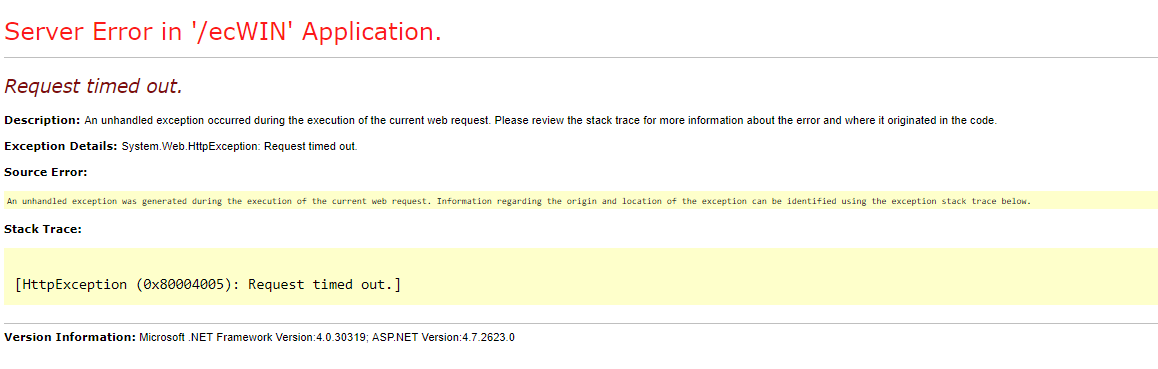
\includegraphics[width=0.8\textwidth]{ecwinerror.png}
        \caption{ecWIN Data Export Error}
        \label{fig:ecwinerror}
    \end{figure}
\end{center}

Thus, the choice of gathering the data from the data editor is chosen, and the method of gathering this data is further discussed in section~\ref{sec:DataGathering}.

% Firstly to download all of the data going back... Then once this has happened, keep downloading the data periodically.
% A system must be in place so that the system can check up on the validity of the data that it has downloaded and compare it to the data on the server. 

\section{Data Conversion} \label{sec:DataConversion}

\section{Data Manipulation} \label{sec:DataManipulation}

\section{Accessibility} \label{sec:Accessibility}

\section{Insights} \label{sec:Insights}


\cite{datasite}

\bibliography{IEEEabrv,References}
\bibliographystyle{IEEEtran}
% \newpage
%\onecolumn
%\appendix


\end{document}